\documentclass [twoside,epsfig,11pt]{jreport}
\usepackage{epsfig}
\usepackage{graphicx}
\usepackage{amsmath}
\usepackage{amssymb}
\usepackage{bm}
\usepackage[dvipdfmx]{color}
\usepackage{listings,jlisting}
\usepackage{url}
\usepackage{verbatim}


\makeatletter
\def\lst@lettertrue{\let\lst@ifletter\iffalse}
\makeatother


%
% %から右側のところはコメント
%
%***************************************************
% 提出用書式
%
\setlength{\topmargin}{5.0mm}		% 表示位置
\setlength{\headheight}{10.0mm}
\setlength{\topskip}{10.0mm}
\setlength{\oddsidemargin}{15.0mm}
\setlength{\evensidemargin}{15.0mm}
\setlength{\textwidth}{145.0mm}
\setlength{\textheight}{215.0mm}
\setlength{\footskip}{10.0mm}
%\setlength{\footheight}{15.0mm}
\renewcommand{\baselinestretch}{1.2}
%

\pagestyle{headings}

%***************************************************

\title{\vspace{-1cm} \Huge 卒業論文 \\
\vspace{1cm}
\huge 小型無線タグを用いた\\
子供の行動計測システム\\
に関する研究 \vspace{3cm}}

\author{
  \begin{tabular}{c}
    {\LARGE{東北大学工学部電気情報物理工学科}}\\
    {\LARGE{張山研究室}}\\ \\
    {\LARGE{斉藤 涼太}}\\
  \end{tabular}
}
\date{}


\begin{document}
\setcounter{secnumdepth}{7}
\maketitle
\large
%\setcounter{page}{2}
\tableofcontents
\chapter{緒言}


\indent
近年,様々な分野でICTの活用が進められ,医療分野における高度な医療の提供,製造業における生産性向上などに貢献している.
一方,保育の分野では,教育の高度化の観点でICTの導入が進んでおらず,保育園に預けた子供の様子を知る手立てが未だ保育士の主観による報告に限られているといった問題が発生している.そのため,子供の行動解析データを介した保育分野におけるICTの導入が求められている.行動解析のために用いるデータにはさまざまあるが,移動場所の傾向を解析することで,同様の移動をした子供のデータから交友関係を,移動場所の傾向から子供の嗜好・個性をつかめる.

以上より,本研究では,子供の移動場所の傾向から行動解析を行うことを目指す.
移動場所の傾向解析を行うには子供がどこにいるのか計測する必要がある.
子供の位置情報を高精度で計測することができれば,子供の移動場所を計測できるが,こちらは設備コストの問題から決定的な技術がまだ登場していない.\cite{ntt}他方,カメラによる記録を解析する手法もあるが,こちらは記録から解析可能なデータにするのが手作業で行われており,解析コストの問題が生じる.そこで,本稿では,設備コスト,消費電力の低い小型無線タグ(TWELITE)を利用して位置計測を自動化することを目的とする.\newline

本論文は以下に示す5章より構成される.

第1章は緒言であり,本研究の背景,目的及び概要について述べたものである.

第2章では本研究で使用したモデルとして,無線タグおよびMQTTプロトコルを用いた計測システムについてまとめた.

第3章では本研究で使用した計測機器であるTWELITEタグの計測精度および使用プロトコルであるMQTTプロトコルの通信の確実性やレイテンシをまとめた.
得られたデータの処理方法についてもここで述べた.

第4章では計測システムを用いて実験を行い,その評価を行った.

第5章は結言である.

以上,本論文の企図するところを概説した.

\chapter{無線タグおよびMQTTプロトコルを用いた計測システム}

\section{はじめに}
この章では今回使用するシステムの構成についてまとめた.

\section{無線タグTWELITE}
\subsection{TWELITEの諸元}
無線タグTWELITEの通信は親機としてMONOSTICK,子機としてTWELITE CUEという機器を使用して行われる.各機器の諸元は表\ref{twelite}の通りである.

親機・子機間の通信は2.4GHz IEEE 802.15.4 に準拠して行われ,変調方式はO-QPSK, DSSSである.\cite{TWdatasheet}
親機MONOSTICKは多数の子機からの情報を受信でき,PCにはシリアルポートとして認識される.
そのため,多くのOSで利用可能である.
子機には加速度センサーが搭載されていて,その測定値を送信することができる.
親機を接続したPC・マイコン等はその情報を確認できるほか,子機から送信された電波がどのくらいの強度で届いたかを後述のLQ値という指標を用いて表示する.\cite{TW1}
子機から親機への送信頻度の設定は加速度サンプリング頻度と加速度送信サンプル数を変化させることにより行え,
サンプリング頻度が25Hz,送信サンプル数が16の時の送信頻度は25/16($\fallingdotseq$1.56)Hzである.
本稿では,電波強度が親機と子機との距離に応じて変化することに着目して実験を行う.

\begin{table}[htb]
 \centering
 \caption{TWELITE諸元}
  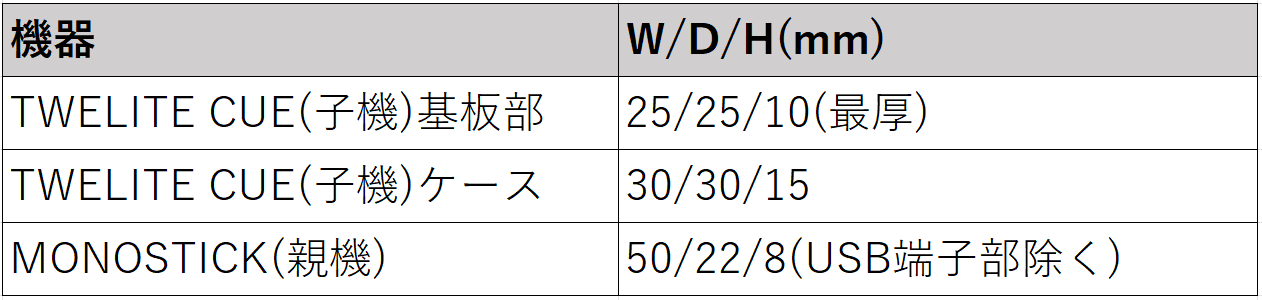
\includegraphics[width = 12cm, bb= 0 0 900 250]{chapter2/TWELITE.png}
   
  \label{twelite}
\end{table}


\subsection{LQ値}
LQ(Link\ Quality)値とはモノワイヤレス社製品における通信品質を表す値で,
LQ値150以上は送信機の近傍にいること,50未満は通信品質が著しく悪いこと(-80dBm)を示す.
以下の式でdBmと変換することができる.\cite{TWLQ}

\begin{equation}
  dBm = (7*LQ-1970)/20
\end{equation}

本研究では,電波強度を評価するための指標としてこのLQ値を用いる.



\section{MQTTプロトコル}
MQTT(MQ\ Telemetry\ Transport)プロトコルは,小型デバイス間でのメッセージ交換用に設計されたTCP/IP(ポート1883)を使用するプロトコルである.
メッセージを確実に送信することを目的としているため,プロトコルヘッダが小さいことが特徴で,即時性,軽量さが長所として挙げられる.\cite{MQTT}
通信環境は,図\ref{mqtt}のように,メッセージを送信する側のパブリッシャと受信する側のサブスクライバに加え,中継者としてのブローカーから構成される.
通信はパブリッシャがブローカーにメッセージを送信し,サブスクライバがブローカーから必要なメッセージを受信するという方式により行われる.
必要なメッセージのみを受信する方法として,TOPICという識別子が用いられている.
パブリッシャはメッセージにTOPICを付加し,サブスクライバは受信するTOPICを設定する.
ブローカーはパブリッシャから受信したデータについて,付加されたTOPICを受信する設定をしているサブスクライバのみにメッセージを送るという仕組みによりサブスクライバが不必要なメッセージまで受信することを防いでいる.
本研究では,MONOSTICKを接続しているマイコン(Raspberry Pi)をパブリッシャ,マイコンとLANを通して接続されたPCをサブスクライバとする.
片方向,かつ集約的な通信を行う本研究において,ブローカーはサブスクライバのPCと兼ねて差し支えないため,
サブスクライバPCにブローカー($\text{Eclipse Mosquitto}^\text{TM}$)を導入して通信を行う.

\begin{figure}[!htb]
  \centering
  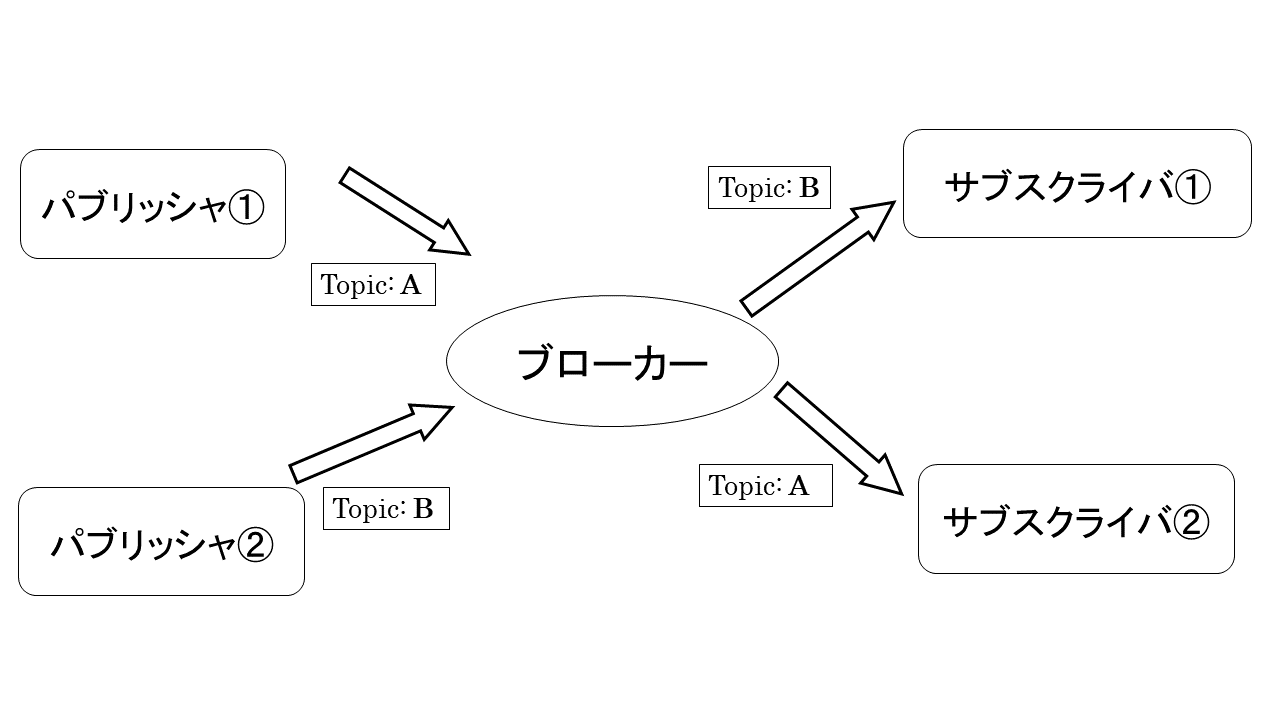
\includegraphics[width = 12cm, bb= 0 0 900 600]{chapter2/MQTT.png}
  \caption{MQTT構成の概要}
  \label{mqtt}
\end{figure}

\clearpage


\section{計測システムの構成}
本研究では,これまでに述べた機器・プロトコルを用いて,プレーパークや保育園において図\ref{system}のようなシステムを構成する.
子供につけたTWELITE無線タグから発信されたデータは,各遊具・遊び場にあるマイコンに接続されたMONOSTICK及びMQTTプロトコルを介して,
子供が”いつ”,”どの遊具・遊び場を使っていたか”がわかるデータとして集積される.
そのうえで,集積されたデータから子供の動きを解析し,個性や交友関係について定量的な分析を行うことを可能にし,より高度な教育につなげることを目指す.



\begin{figure}[!htb]
  \centering
  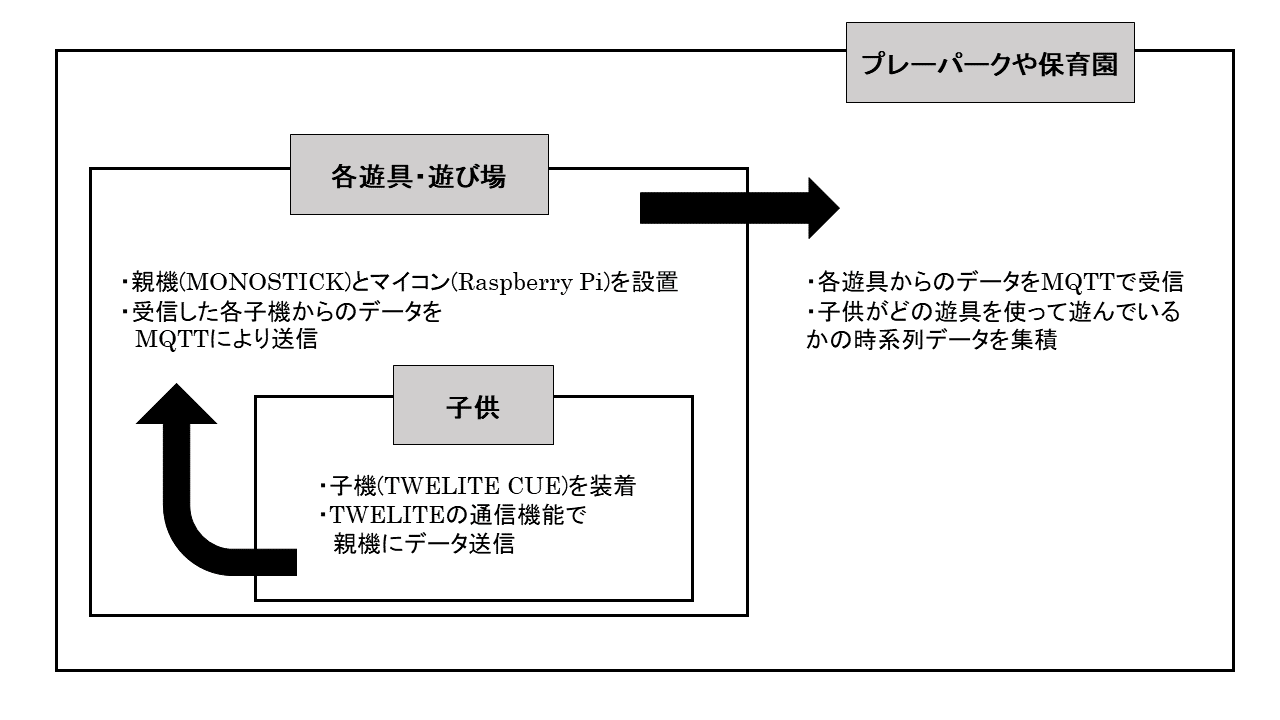
\includegraphics[width = 15.8cm, bb= 0 0 1000 600]{chapter2/kouseigaiyou.png}
  \caption{計測システムの構成}
  \label{system}
\end{figure}









\chapter{システムの性能評価}\label{chap3}
\section{はじめに}
本章では2章で示したシステムの機器・プロトコルについて,実環境での使用を目標とした性能評価を行った.
また,測定に伴い発生する欠測値の補間方法ならびにノイズの除去方法についても考察・実証のうえまとめた.

\section{TWELITE無線タグの性能評価}\label{TWELITEs}
ここでは,システムのうち,TWELITE無線タグについて,実際の通信距離と電波強度の関係についてまとめた.

\subsection{通信距離と電波強度の関係の定量的な測定}
\subsubsection{測定の条件}
本測定ではMONOSTICKをPCに接続し,MONOSTICKとTWELITE CUEを使用して行った.
周囲に何もない屋内環境(体育館)において,MONOSTICKとTWELITE CUEの距離を1m,2m,3m,4m,5m,10m,15m,20m,25mに固定し30秒間測定した.
測定は2つのTWELITE CUEタグを使用して行い,発信頻度は1.56Hz(加速度サンプリング頻度25Hz,送信サンプル数16)とした.
測定時間30秒間に送られてくる電波強度(LQ値)を平均し,測定結果とした.


\subsubsection{測定結果}
通信距離と電波強度の測定結果は図\ref{LQ25}のようになった.
電波強度は通信距離5mまでは一次関数的な減少を見せたが,その後は多少の上下こそあるもののほぼ横ばいの推移を見せた.


\begin{figure}[!htb]
  \centering
  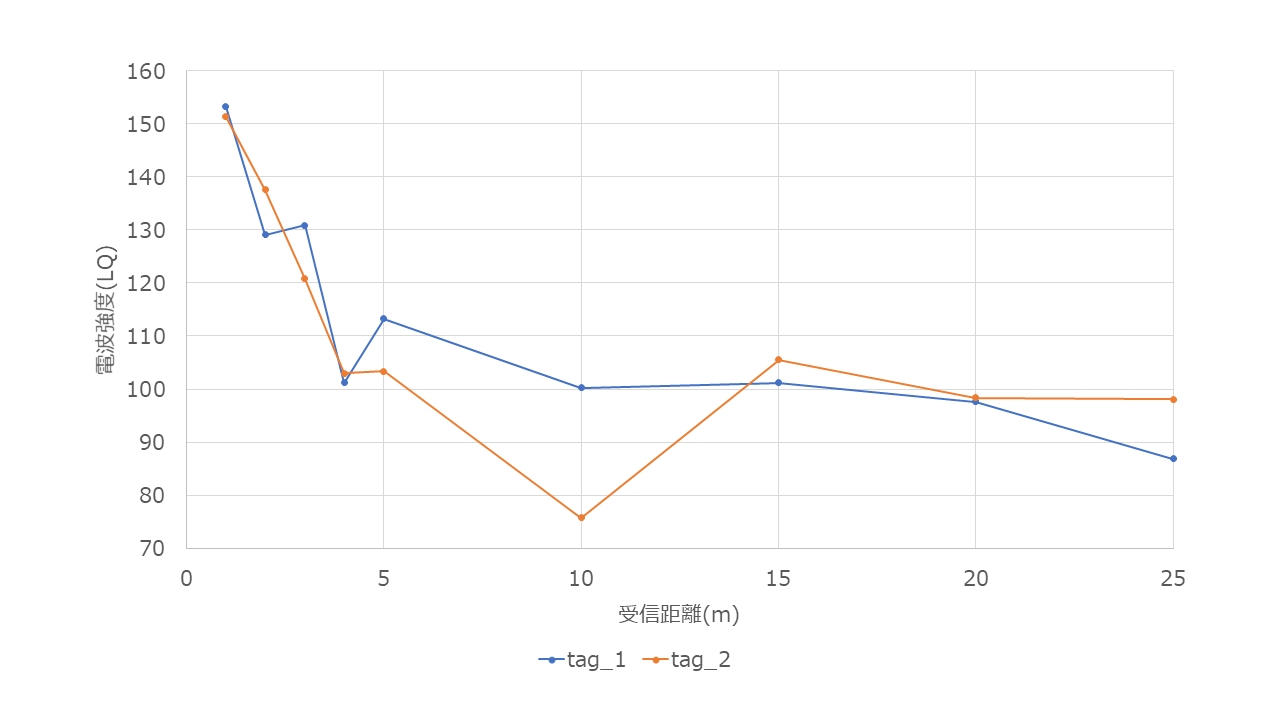
\includegraphics[width = 15cm, bb= 0 0 1000 600]{chapter3/LQ25.png}
  \caption{通信距離と電波強度の測定結果}
  \label{LQ25}
\end{figure}
\clearpage


\subsubsection{測定結果からの考察}
以上の結果より,特異的な結果は通信距離おおむね5m以内で現れるLQ値120以上という値であることが分かった.
よって,以降の研究では通信距離が5m以内となる計測条件を設定して実験を行うこととする.


\subsection{機器の評価を踏まえたTWELITE無線システムの利用方法}
以上の評価結果を踏まえ考えられるTWELITE無線システムの利用方法は以下の通りである.
図\ref{LQ25}からわかるように,TWELITE無線の電波強度は,通信距離5m程度までは単調に減少し,それ以降は横ばいの推移をとる.
このことを用いて,MONOSTICKとTWELITE CUEが5m以下の距離にあるような使い方をする.

\subsubsection{網羅的配置}
まず,MONOSTICKを取り付けたマイコンの配置について,一つのMONOSTICKが受け持つ範囲は,
半径5m以下の円形の範囲とする.
そのうえで,図\ref{sysmodel}のようにカバーしたい範囲を網羅するように配置することで,
子供がいずれかのMONOSTICKと5m以内に近接していることになるので,高い電波強度を示すMONOSTICKが必ず現れる.
それにより子供の位置を概ね特定することができる.
この方法では,値による閾値を示さずとも他との比較により位置を推定できるので簡単である.
\clearpage

\begin{figure}[!tb]
  \centering
  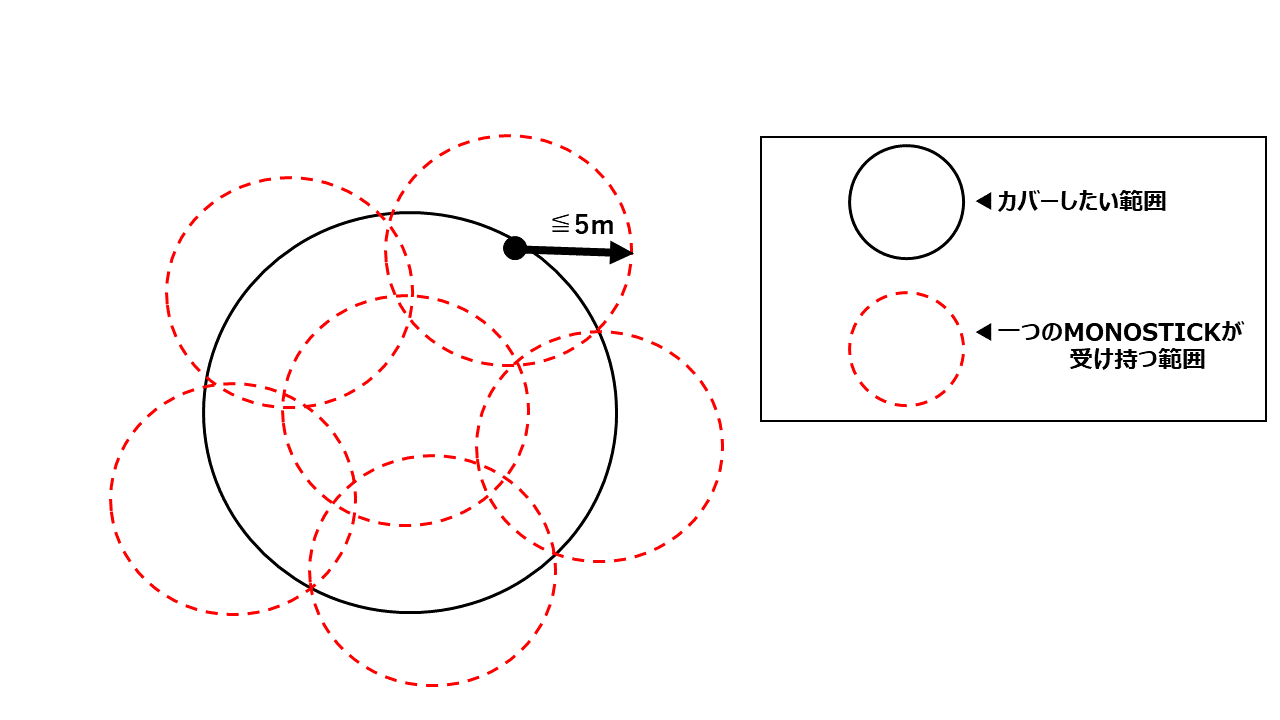
\includegraphics[width = 16cm, bb= 0 0 1000 700]{chapter3/sysmodel.png}
  \caption{MONOSTICKの網羅的配置}
  \label{sysmodel}
\end{figure}



\subsubsection{チェックポイント的配置}
MONOSTICKが受け持つ範囲は同様に半径5m以下とする.
ここで,MONOSTICKが受け持つ範囲の中に,特定の入口・出口ゲートや,滑り台の降り口など,
特定の遊びをしたときに通るポイントを含めることにより,子供が何をしていたかを概ねつかむことができる.
使用するMONOSTICK,マイコンの量を減らせるので,リソースに限りがあるときに有用である.

\clearpage


\section{MQTTプロトコルの性能評価}
つづいて,MONOSTICKを取り付けた複数のマイコンからデータを集約するためのMQTTプロトコルについて評価を行う.
MQTTプロトコルは軽量かつ即時性に優れたプロトコルであるが,実際の使用環境におけるデータの送受信に耐えるか確かめるべく
データ受信のレイテンシや送受信の成功率についてまとめた.

\subsection{測定環境}
MQTTのパブリッシャとしてはMONOSTICKを取り付けたマイコン(Raspberry Pi)を使用し,
ブローカーおよびサブスクライバPCとしてWindows PC1台を使用した.
なお,MQTTはポート1883を使用したTCP/IP通信によって行われる.
LANによる接続はすべてWi-Fiを用いた無線通信により行うこととし,それを実現するためのWi-Fiルーター1台も用いた.
Wi-Fiは屋外利用が想定されることおよび安定した通信を目指すことから2.4GHz帯を使用した.
実際に使用したMQTTの構成詳細を図\ref{MQTTprop}に示した.

なお,本測定で使用したタグからのデータ取得及びMQTTデータ転送のプログラムについて,ソースコードは最後に付録としてまとめてある.

\clearpage

\begin{figure}[htb]
  \centering
   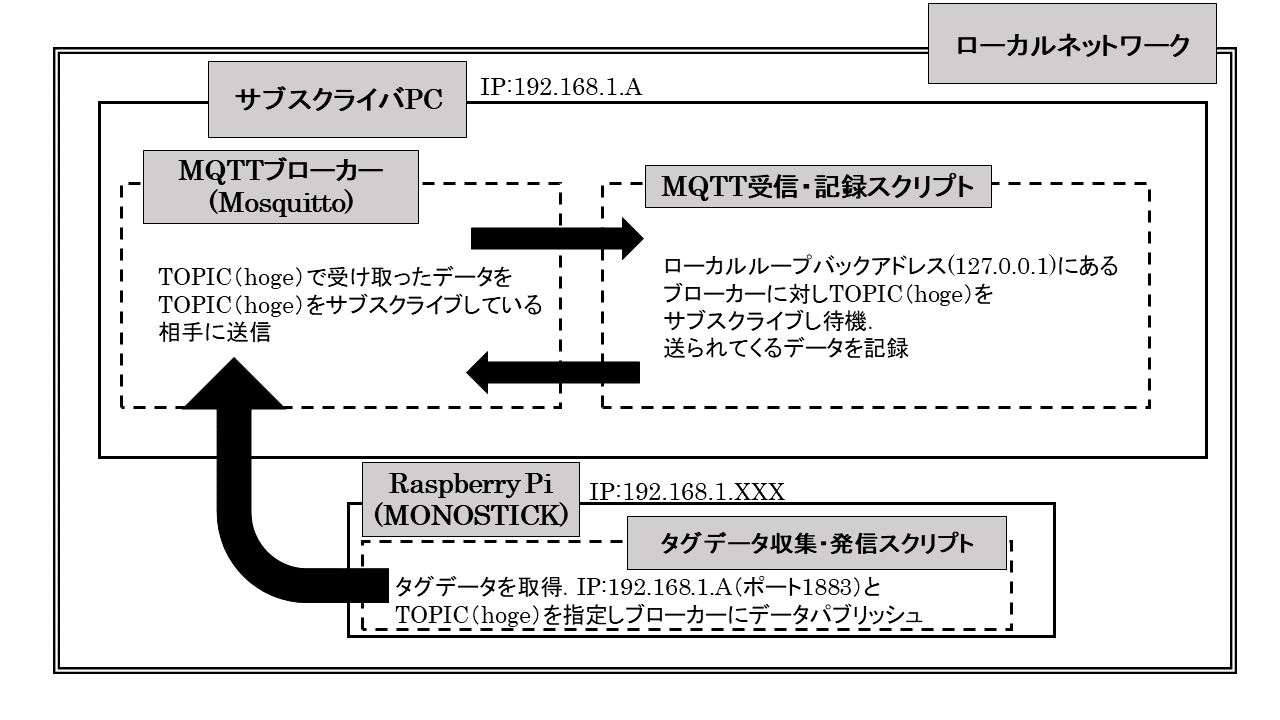
\includegraphics[width = 15.8cm, bb= 0 0 1000 600]{chapter3/MQTTprop.png}
   \caption{MQTTによるやり取りの詳細}
   \label{MQTTprop}
\end{figure}


\subsection{MQTTの受信成功率測定}
受信成功率の測定はMONOSTICKから取得したTWELITE CUEタグからの受信データ(34 Byte)をMQTTプロトコルによって送信する際,パブリッシャ側のマイコンでも同時にログをとることにより行った.
MQTTを介してサブスクライバ側が受け取ったデータとパブリッシャ側に残るデータを照らし合わせ,
データの欠測のうちMQTTプロトコルに起因する欠測の数を計測し受信成功率を求めた.
試行回数6879回のうちMQTTプロトコルに起因するデータの欠測は0件だったため,MQTTの受信成功率は100\%であることが確かめられた.
\clearpage

\subsubsection{時刻の同期に関する問題のMQTTによる解決}
本研究では,複数のマイコンを用いてデータの取得を行うが,複数のマイコンの時刻がずれていると
マイコンごとにTWELITE CUEからのデータ受信時刻が異なることになり,正確な受信時刻を得ることができない.
それを防ぐためには,マイコンの時間を同期する必要があった.
しかし,MQTTが即時性に優れたプロトコルであることを利用して受信時刻をサブスクライバ側のPCの時刻に一括することができれば,
マイコンの時間を同期する必要がなくなる.
本稿ではそのための条件を設定して実験を行った.

\subsection{MQTTのレイテンシ測定}
本研究で送信されているデータの送信頻度は1.5Hz程度である.
よって,レイテンシを0.5秒以内に抑えることができれば前後のデータが入れ替わることなくマイコンの時刻同期をせずとも受信時間に正確さが出る.
本稿では,様々な条件のもとでMQTTプロトコルのレイテンシを測定し,実際に0.5秒以内に抑えられているか確かめた.

\subsubsection{単一パブリッシャからの受信で測定したレイテンシ}
受信成功率と同様にしてMQTTのレイテンシ測定を行った.
レイテンシ測定はパブリッシャのマイコンとサブスクライバのPC双方にMONOSTICKを取り付けることによって行った.
TWELITE CUEから発信されたデータは,パブリッシャのマイコンに取り付けられたMONOSTICKおよびMQTTを介してサブスクライバのPCに届く.
サブスクライバPCでは,MQTTを介してデータが届いた時刻を記録した.
一方,サブスクライバのPCでも同じデータをMONOSTICKのみを介して取得し,その時間も記録した.
その二つの受信時間を比較すればMQTTの遅延時間を求めることができる.
レイテンシの計測結果は以下の表\ref{mqttlate}のようになった.
最大値こそ4秒台と大きいものの,平均,標準偏差ともに小さく抑えられていることからわかる通り,ほとんどの場合では非常に小さい値になっていることが特徴である.

\clearpage

\begin{table}[htb]
 \centering
  \caption{単一パブリッシャからの受信で測定したレイテンシ}
  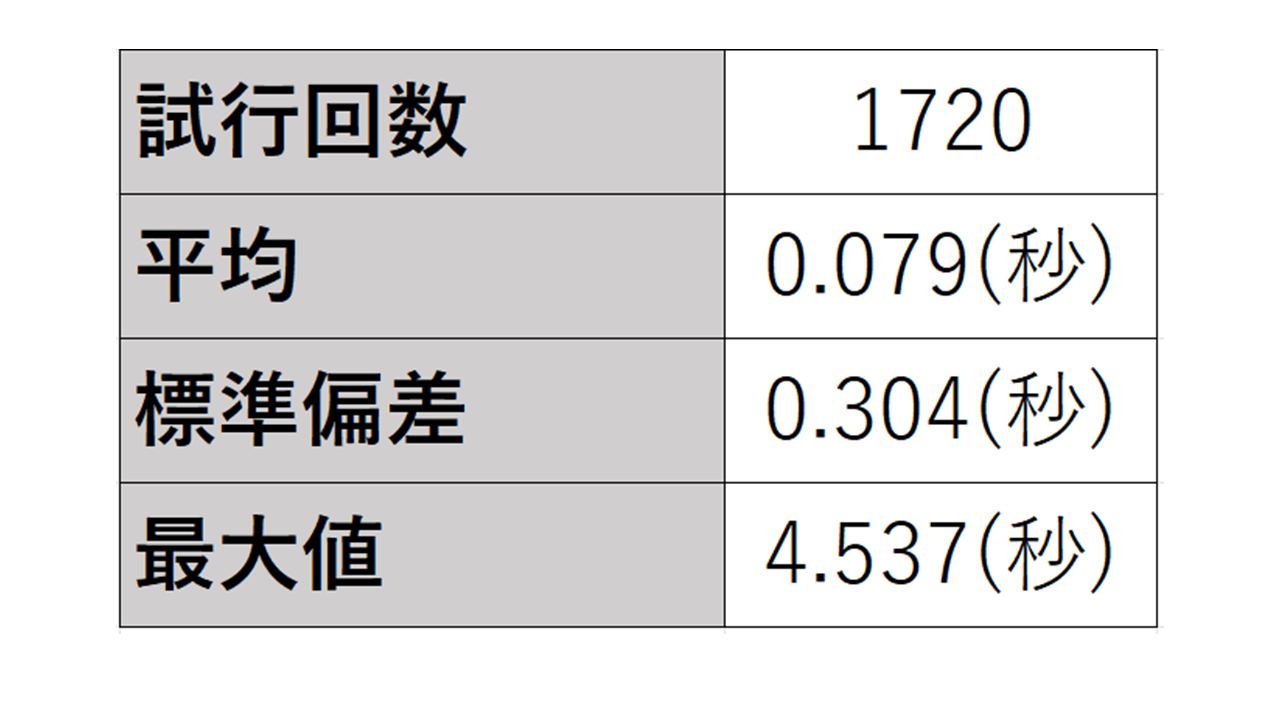
\includegraphics[width=7cm, bb= 0 0 1200 600]{chapter3/mqttlate.png}
  \label{mqttlate}
\end{table}

\subsubsection{複数パブリッシャからの受信で最速をとったレイテンシ}
本研究で想定されているシステムではTWELITE CUEからのデータは複数のマイコン・MQTTパブリッシャを通して届く.
そのため,複数のパブリッシャから送られた同一時刻の情報のうち,一番最初にサブスクライバに届いた時刻を代表として記録すればレイテンシを抑えることができる.
4台のマイコンを用意し,それぞれにMONOSTICKを取り付け,同一のサブスクライバに向けてMQTTで情報を送信した.
単一パブリッシャでの実験と同様に,MQTTを通してサブスクライバに届いた時刻を記録し,同一データに関する時刻のうち一番早いものを比較のための代表時刻とした.
サブスクライバのPCにもMONOSTICKを取り付けTWELITE CUEからのデータを記録し,受信時間を比較しレイテンシとした.
レイテンシの計測結果は以下の表\ref{mqttlate2}のようになった.
最大レイテンシは0.5秒以下に抑えられているため,本研究ではマイコンの時刻の同期は行わず,記録する時刻はMQTT受信後のサブスクライバの時刻とする.

\begin{table}[htb]
  \centering
   \caption{複数パブリッシャからの受信で測定したレイテンシ}
   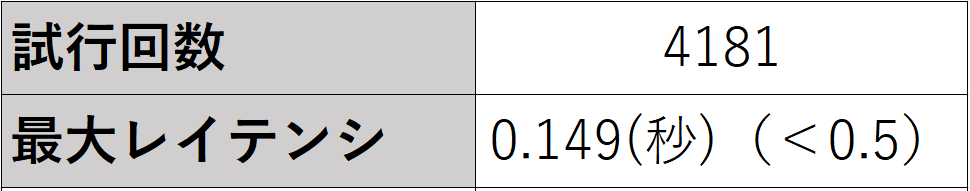
\includegraphics[width=7cm, bb= 0 0 800 250]{chapter3/mqttlate2.png}
   \label{mqttlate2}
\end{table}

\clearpage

\section{データの処理方法の決定}
ここでは,TWELITEタグ及びMQTTプロトコルを用いて集約されたデータに発生するノイズの除去や欠測値の補間について述べる.

\subsection{状態空間モデルを用いたフィルタの適用}
一般に,あるシステムを運用する際に,実際にはシステムの状態を直接確認できず,環境や観測機器によるシステムノイズや観測ノイズが生じる.
このノイズはある分散をもった正規分布に従うと仮定してフィルタリングすることができ,計量や信号処理などの分野で活用されている.
本研究で得られる測定結果も,電波干渉等に影響され得られるデータには振動が生じているため,状態空間モデルを用いたフィルタを使用しノイズを除去する.
フィルタリングは以下の式\ref{kal1},\ref{kal2}に基づいて行われる.
\begin{equation}
 \label{kal1}
 x_n = Fx_{n-1} + Gv_n 
\end{equation}

\begin{equation}
  \label{kal2}
  y_n = Hx_n + w_n
\end{equation}

ここで,
\it
F,G,H
\rm
は適切な次元を持つ行列で,
\it
$v_n$,$w_n$
\rm
は平均0でそれぞれ$\tau^2$,$\sigma^2$
を分散とする正規分布に従うとする.\cite{TSSS}
状態空間モデルでは,時間更新(Predict)により$x$の一歩先の状態を予測し,実際の観測値$y$によって推定値の更新(Correct)を行う.\cite{kalman}
本稿では,これを利用し,適切な$\tau^2$の値を用いることで$x$の状態を推定する.
図\ref{kalman}は測定されたデータセットに対し$\tau^2 = 0.1$としてフィルタリングした結果である.
得られた測定値の特徴を残しつつノイズの除去が行われている.

\clearpage
\begin{figure}[!t]
  \centering
  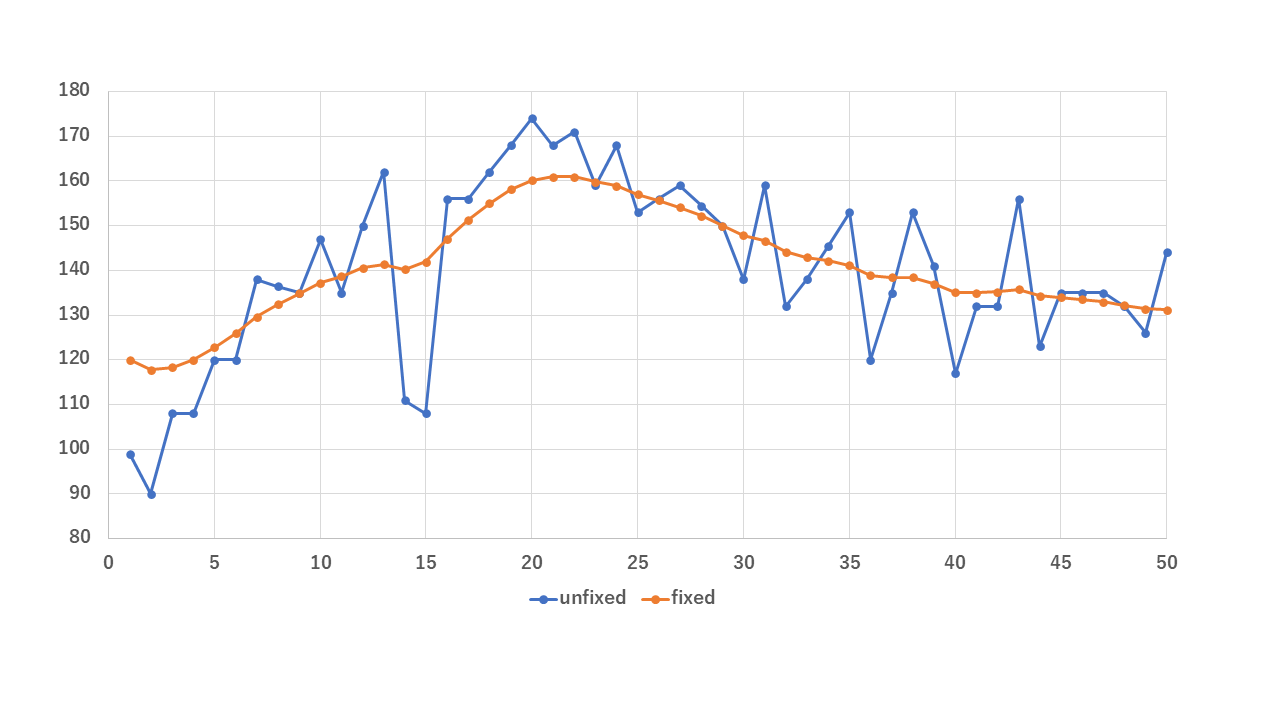
\includegraphics[width = 15cm, bb= 0 0 1000 500]{chapter3/kalman.png}
  \caption{状態空間モデルを用いたフィルタリング結果}
  \label{kalman}
\end{figure}



\subsection{欠測値の補間方法}
前述した状態空間フィルタを適用するためにはデータを時系列データとする必要がある.
しかし,TWELITE CUE・MONOSTICKを用いた実験では,データの発信頻度にかかわらずデータの欠測が生じる.
複数のMONOSTICKを使用して同一のデータを複数経路で受信している場合,
受信しているうちの一部が欠測により不足していることがある.
この場合,正しい比較ができなくなるため適切な方法で欠測を補間する必要がある.
ここでは,適切に補間するための方法について検討する.

\subsubsection{NN補間}
NN(Nearest\ Nearby)補間は,一番単純な補間方法で,欠測が発生した部分の前後
のデータのうち,該当部に近いほうのデータを用いてそのまま補間する.

\subsubsection{線形補間}
線形(linear)補間は,欠測が発生した部分の前後のデータ間で,値が線形な変化をしたと仮定し,その値で補間する方法である.

\subsubsection{スプライン補間}
(三次)スプライン(spline)補間は,N個の測定点(データ)が与えられたデータセットをN-1個の区間に分割し,その区間ごとに適切な三次曲線を求めてそれをもとに補間する方法である.
区間ごとの三次曲線は以下の条件を満たす.
\begin{quote}
  \begin{itemize}
   \item 各区間を補間する曲線はその両側の点を通る.
   \item N個の各点において両側の区間の1次導関数は等しい.
   \item N個の各点において両側の区間の2次導関数は等しい.
  \end{itemize}
\end{quote}
三次曲線の未知数4つに対して,式が4つできるのでこの条件により各区間ごとに補間する曲線の式が求まることを利用し補間するのがスプライン補間である.

\subsection{補間方法の比較}
先に述べた三つの補間方法の比較のため,実際に計測できたデータセットからランダムに一部を削除し,
欠測のある状態を作り出した.そのうえで実際の計測データ(unfixed)とそれぞれの補間方法で補間されるデータを示したのが図\ref{interp}である.
まず,スプライン補間は,各測定点の両側で1次導関数,2次導関数が等しいという条件に影響され,データの上下が激しい区間で欠測した場合に
オーバーシュートが発生するため,補間方法として適切ではないことが分かった.
よって,線形補間とNN補間に絞って比較した.
この二つの補間方法による差は大きくないが,実際の子供の移動により近いと考えられるのは線形補間であるため,本稿では線形補間により補間を行うこととする.

\begin{figure}[!htb]
  \centering
  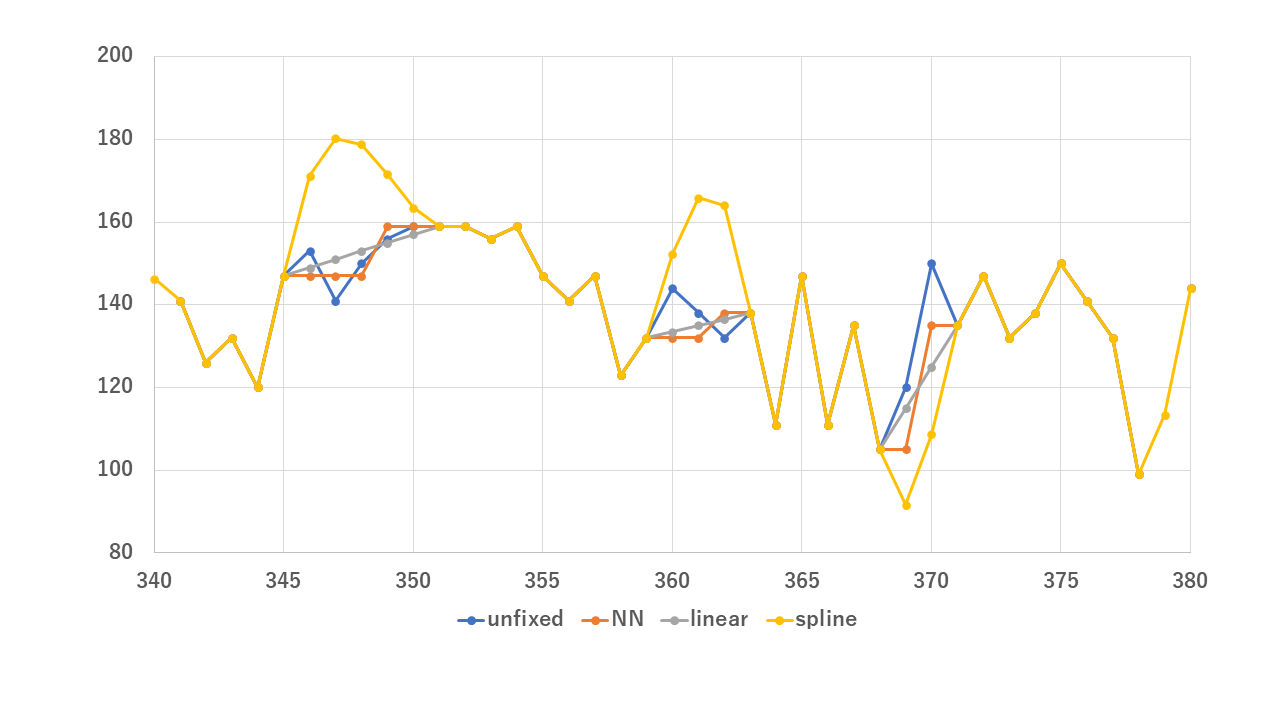
\includegraphics[width = 15cm, bb= 0 0 1000 600]{chapter3/interp.png}
  \caption{補間方法の比較}
  \label{interp}
\end{figure}



\chapter{システムを用いた実験,評価}

\section{まえがき}
ここでは,観測者であるTWELITE CUEタグの位置の推定を目指し,第\ref{chap3}章において評価したシステムを用いて簡単な実験を実施した.
その実験の結果と評価についてまとめる.

\section{実験の概要}

\subsection{測定機器}
先述のTWELITE CUE,MONOSTICKのほかに,サブスクライバPCとしてMQTTブローカーMosquittoを導入済みのWindows PC1台,
MQTTプロトコル(TCP/IP)を実現するためのWi-Fiルーター1台を用いて行った.


\subsection{実験環境}
図\ref{TWjikken}に実験環境の写真を示した.
室内で180cm四方の机を囲むような環境になっているが,机を用いたのはMONOSTICKについて,床から離して設置するよう推奨されているためである.
MONOSTICKを取り付けたマイコン(Raspberry Pi)は机の四隅に設置されている.
同様に床から離すよう推奨されているTWELITE CUEタグは,自由に動くプラスチック製のワゴンに置かれ,そこから発信されたデータは4か所のMONOSTICK・MQTTプロトコルを介してサブスクライバPCに集約されるようになっている.


\begin{figure}[htb]
  \centering
   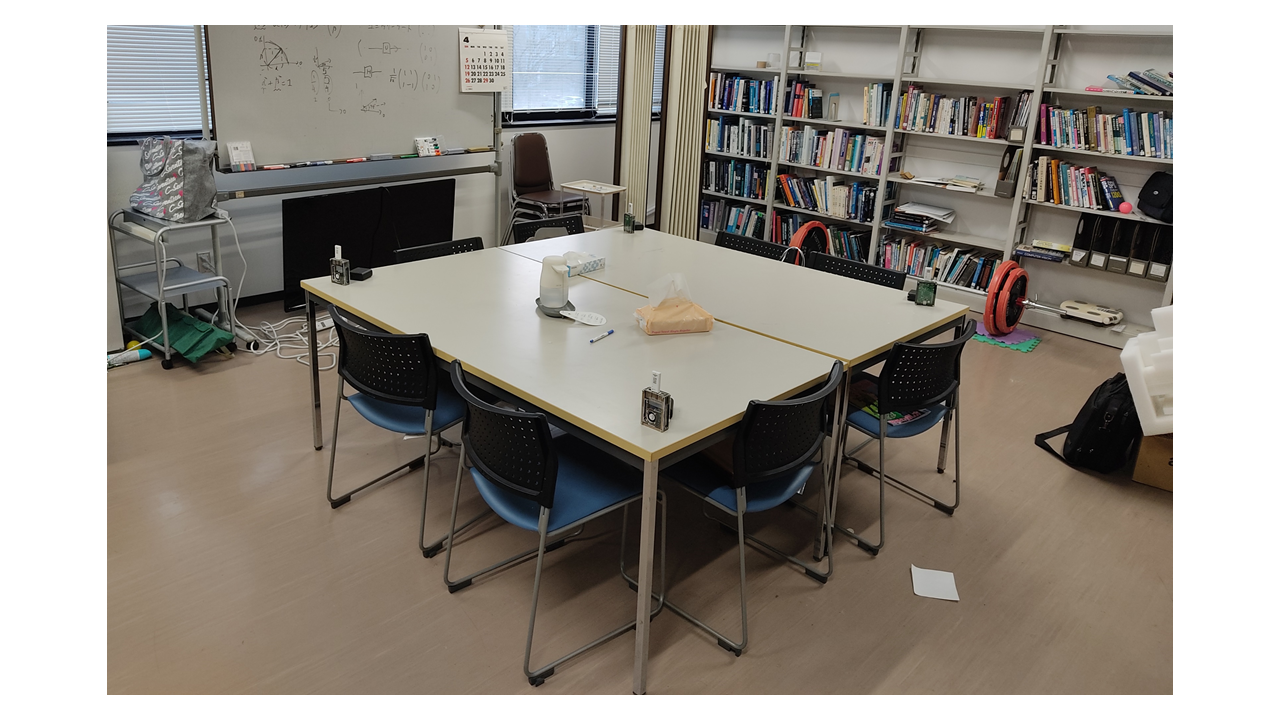
\includegraphics[width = 15cm, bb= 0 0 1000 600]{chapter4/TWjikken.png}
   \caption{実験環境の写真}
   \label{TWjikken}
\end{figure}


\subsection{実験方法}

\begin{enumerate}
  \item 机の四隅に置かれたMONOSTICK・Raspberry PiからサブスクライバPCにMQTTでデータが送られるよう設定する.
  \item 1.56Hz(加速度サンプリング頻度25Hz,送信サンプル数16)でデータを送信するよう設定したTWELITE CUEタグを置いたプラスチックワゴンを机を回るように自由に移動させる.
  移動の様子は同時にビデオ撮影を行って記録しておく.
  \item サブスクライバPCで,集約されたデータに線形補間による補間と状態空間モデルによるフィルタリングを行ったのち比較を行い,観測者から一番近いMONOSTICKが4台のうちどれであるか求める.
  \item ビデオ撮影によって得られた情報と比較を行い,今回のシステムによる推定の正解率を調べる.
\end{enumerate}


\section{実験結果}
実験中192回のデータ送信があったうち,システムによって得られた推定の正解は174回であり,正解率は90.6\%であった.
不正解となった約10\%のデータは約5秒程度の連続した不正解であった.

\section{実験の評価}
システムによる推定の正解率が高く,システムの近距離の判別性能は高いといえる.
不正解となった時間について,その時間はどのMONOSTICKにも極度に接近していない状態であった.
そのため,不正解の一因としては,最も近いタグとそれ以外のタグとの距離比があまりないために電波強度に差が生まれず,システムが推定を誤ったと考えられる.












\chapter{結言}
本稿では,子供の移動場所の傾向を解析して行動解析を行うという目標のもと,小型無線タグTWELITEを用いた位置情報推定に向け,機器の性能評価と転送プロトコルの提案,補間やフィルタリングを含めたシステムの構成と性能評価を行った.
まず,小型無線タグの性能評価においては,通信距離と電波強度の関係について,ある一定の距離(5m程度まで)は通信距離の増加に伴い電波強度が減少するがそれ以降は電波強度が横ばいになるという結果が得られた.
続いて,MQTTプロトコルについて,0.5秒以下の低レイテンシで確実性の高いプロトコルであることが確かめられ,本稿における転送プロトコルとしては十分な性能を示した.
小規模な屋内で実装したシステムの性能評価では,90.6\%という高い推定正解率を示し,子供の移動場所の傾向を示すためには十分な結果と考えられる.
推定不正解となった部分についても,距離比の差が小さいことに起因するため,今後大きな規模に拡大することにより改善することも考えられる.
本稿ではデータ処理について,状態空間モデルを用いたフィルタリングおよび線形補間を用いたが,フィルタや補間方法には今回検討したよりも多くの方法・ソースコードがあるため,その中から最適なものを検討していきたい.
また,今回は小規模な実験にとどまったが,今後さらに実験環境を広げた場合の実験も行っていきたい.
本研究の最終目標はプレーパーク,保育園等での子供の位置情報を推定し,その情報を集積・分析することである.
実際の測定環境はきれいな図形のような形をしているとは限らず,システムの性能評価を踏まえたカスタマイズが必要となるので,それも併せて取り組んでいきたい.
そのうえで,集積されたデータの解析を含めた解析をして評価可能なシステムとして提案したい.


\renewcommand{\bibname}{参考文献}
\begin{thebibliography}{8}
\bibitem{ntt} 株式会社NTTデータ,谷沢幹也. "屋内測位のニーズと技術紹介", \url{https://inforium.nttdata.com/trend\_keyword/264.html}, 2017-07.
\bibitem{TWdatasheet} モノワイヤレス株式会社 "TWELITE CUE データシート", \url{https://twelite.gitbook.io/mw-psd-cue/}
\bibitem{TW1}大澤文孝 "TWELITEではじめる「センサー」電子工作" 工学社 2019-06
\bibitem{TWLQ}モノワイヤレス株式会社 "TWELITE CUE 製品情報", \url{https://mono-wireless.com/jp/products/twelite-cue/index.html}
\bibitem{MQTT} IBM "MQTTプロトコル", \url{https://www.ibm.com/docs/ja/ibm-mq/8.0?topic=ssfksj-8-0-0-com-ibm-mq-pro-doc-q002870--htm}
\bibitem{TSSS} The Comprehensive R Archive Network "Package TSSS", \url{https://cran.r-project.org/web/packages/TSSS/TSSS.pdf}
\bibitem{kalman} MathWorks "カルマンフィルタ", \url{https://jp.mathworks.com/discovery/kalman-filter.html}
\bibitem{pal} モノワイヤレス株式会社 "パルスクリプト", \url{https://mono-wireless.com/jp/products/TWE-APPS/App_pal/palscript.html}
\end{thebibliography}

\chapter*{謝辞}

本研究を進めるにあたり,多くの皆様にたくさんの協力,助言をいただきました.\par
主指導教員である張山昌論教授には,日々の討論などでデータの取り方,まとめ方から研究に対する姿勢に至るまで鋭い指摘や多くの助言をいただきました.
また,研究室において安心して,集中して研究をできるよう気にかけていただきました.
心より感謝申し上げます.\par
副指導教員であるハシタムトゥマラウィッデヤスーリヤ准教授には,研究活動だけでなく,日々の研究室生活において充実した研究生活を送れるように多くの支援,助言をしていただきました.
心より感謝申し上げます.\par
また,小柴満美子准教授および小山高専の小林康浩先生にも,実際のプレーパークでの経験や機器の使用経験からのありがたい助言,サンプルプログラムの提供など,様々な面でサポートいただきました.
心より感謝申し上げます.\par
最後に,研究会や日々の議論におきまして親睦を深めともに研鑽しあった同期をはじめ,多くのご助言を頂きました張山研究室の皆様に感謝申し上げます.\par
\begin{flushright}
  令和4年3月24日
\end{flushright}

\appendix
\chapter{付録}
\indent
付録として,MQTTパブリッシャ側のプログラム(TWELITE CUEタグ)からのデータ取得プログラム(\ref{scpub}),MQTTサブスクライバ側のプログラム(\ref{scsub})のソースコードを記載した.
実行環境はPython3.10.1である.
なお,パブリッシャ側のプログラムはモノワイヤレス株式会社のパルスクリプトを改変したものである.\cite{pal}


\lstset{
  basicstyle={\ttfamily\scriptsize},
  commentstyle = {\itshape\scriptsize},
  %identifierstyle={\small},
  %keywordstyle={\small\bfseries},
  %dkeywordstyle={\small},
  %stringstyle={\small\ttfamily},
  frame={tb},
  breaklines=true,
  columns=[l]{fullflexible},
  numbers=left,
  xrightmargin=0zw,
  xleftmargin=3zw,
  numberstyle={\scriptsize},
  stepnumber=1,
  numbersep=1zw,
  lineskip=-0.5ex
}



\lstinputlisting[caption=パブリッシャ側プログラム,label=scpub]{Appendix/mqttpubthesis.py}

\clearpage
\lstinputlisting[caption=サブスクライバ側のプログラム,label = scsub]{Appendix/mqtt_subtestthesis.py}

\end{document}






